\documentclass[letterpaper,headings=standardclasses,parskip=half]{scrartcl}

% \usepackage[french]{babel}
\usepackage[hmargin=1.25in,vmargin=1in]{geometry}
\usepackage{graphicx}
\usepackage[hidelinks]{hyperref}
% \usepackage[backend=bibtex]{biblatex}

% \addbibresource{references.bib}

\titlehead{
    \centering
    
\includegraphics[width=2in]{Signature_electronique 150.jpg}
}
\subject{LOG8415E - Advanced Concepts of Cloud Computing}
\title{Final Project – Scaling Databases and Implementing Cloud Design Patterns}
\subtitle{Report}
\author{Nam VU (2230468)}
\date{\today}
\publishers{Polytechnique Montréal – Fall 2023}


\begin{document}

\maketitle
\thispagestyle{empty}

\clearpage
\pagenumbering{arabic}

\tableofcontents

\clearpage

\section*{Handover Documentation Report}

\subsection*{Project Title}

Scaling Databases and Implementing Cloud Design Patterns

\subsection*{Report Date}

\today

\subsection*{Team Members}

\begin{itemize}
    \item Nam Vu (2230468)
\end{itemize}

\noindent\rule{\textwidth}{0.3pt}

\section*{Executive Summary}

In this last lab assignment, we are asked to setup a MySQL cluster on Amazon EC2 and implement two Cloud patterns: Proxy and Gatekeeper.
We reused and extended the codebase from the previous projects to setup and configure the AWS infrastructure programmatically using Python and boto3. Details of the implementation and benchmarking results are presented in the following sections.

\noindent\rule{\textwidth}{0.3pt}

\section{Introduction}

Deploying a database on the cloud is a common task in the industry. A cluster deployment is often preferred over a standalone server for better performance and availability. In our setup, the implementation of two Cloud patterns, Proxy and Gatekeeper, offers additional performance and security benefits.

\section{Project Objectives}

Different objectives are fixed for this project:

\begin{itemize}
    \item Deploy MySQL on Amazon EC2 in two different configurations: standalone server and cluster.
    \item Benchmark the performance of the two deployments with sysbench.
    \item Implement two Cloud patterns: Proxy and Gatekeeper.
\end{itemize}

\section{Approach}

As with the other assignments, we use Python and boto3 to setup and configure the AWS infrastructure. In addition, we also rely this time on Jinja2 to template the diverse shell scripts used to setup the Ubuntu 22.04 EC2 instances depending on their roles. All Python dependencies are managed with Poetry and the project is version-controlled with Git.

\section{Tasks and Responsibilities}

\subsection*{Nam Vu}

\begin{itemize}
    \item MySQL deployments
    \item Benchmarking
    \item Patterns implementation
\end{itemize}

\section{Progress and Achievements}

All architectures can be easily deployed following the instructions in the \texttt{README.md} file of the project repository.

\subsection{MySQL deployments}

In this section we deploy MySQL in two different configurations: standalone server and cluster. We then also load the \texttt{sakila} sample database into both deployments.

\subsubsection{Standalone server}

\textbf{Directory: \texttt{src/standalone}}

\begin{figure}[h]
    \centering
    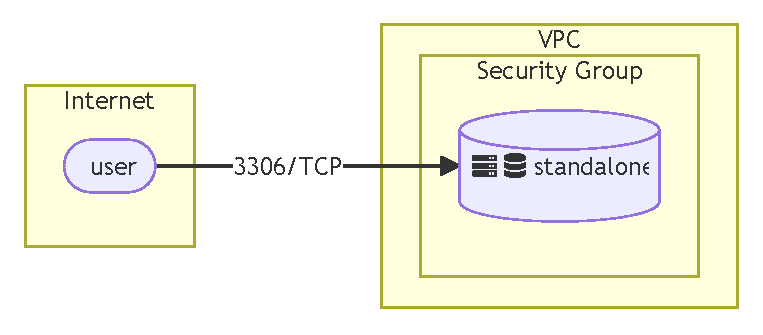
\includegraphics[width=0.5\linewidth]{figures/standalone.mmd.pdf}
    \caption{Standalone MySQL server}
    \label{fig:standalone}
\end{figure}

In this simple configuration, we deploy a single \textit{t2.micro} instance running Ubuntu 22.04 and install the latest version of MySQL Server from the system APT repositories.

We allow remote connections to the database by modifying the \texttt{bind-address} option in the MySQL configuration file and update the root password. We also open the port 3306 on the AWS security group to allow incoming connections from the Internet.

Finally, we load the \texttt{sakila} sample database using the \texttt{mysql} command-line client.

Figure~\ref{fig:standalone} illustrates this configuration.

\subsubsection{Cluster}

\textbf{Directory: \texttt{src/cluster}}

\begin{figure}[h]
    \centering
    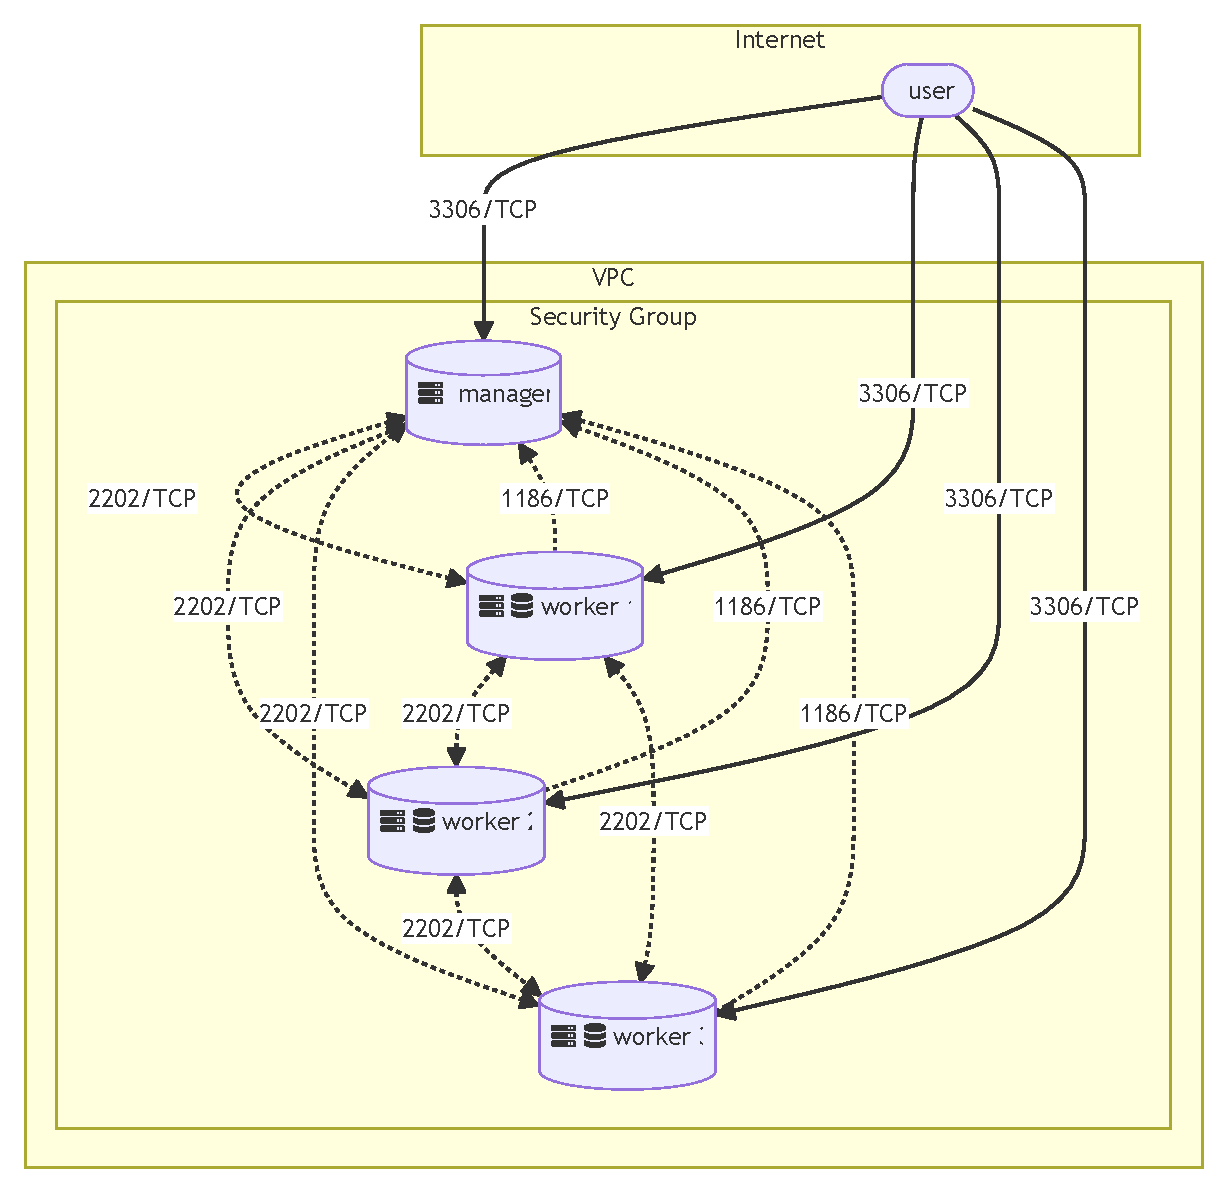
\includegraphics[width=0.75\linewidth]{figures/cluster.mmd.pdf}
    \caption{MySQL cluster}
    \label{fig:cluster}
\end{figure}

This configuration requires four \textit{t2.micro} instances running Ubuntu 22.04.

First, we need to setup the official MySQL APT repository that provides cluster-compatible packages on all instances.

Then, we install the required packages on each node:
\begin{itemize}
    \item Manager node: \texttt{mysql-cluster-community-management-server} (\texttt{mgmd} service, 1186/TCP) and \texttt{mysql-cluster-community-server} (\texttt{mysqld} service, 3306/TCP)
    \item Worker node: \texttt{mysql-cluster-community-data-node} (\texttt{ndbd} service, 2202/TCP) and \texttt{mysql-cluster-community-server} (\texttt{mysqld} service, 3306/TCP)
\end{itemize}
\texttt{mgmd} will coodinate the cluster from the manager node while \texttt{ndbd} will store the data on worker nodes. The \texttt{mysqld} service is installed on all nodes to allow API access to the database.

Using Jinja2 templates, we dynamically generate the configuration files for each node and copy them to the appropriate location.

We also load the \texttt{sakila} sample database on each node and open the port 3306 on the AWS security group to allow incoming connections from the Internet.

Figure~\ref{fig:cluster} illustrates this configuration.

\subsection{Benchmarking}

\textbf{File: \texttt{tools/benchmark.sh}}

For the benchmarking, we use the \texttt{sysbench} tool to generate a workload on the database. We chose the \texttt{oltp\_read\_write} test that simulates a mixed OLTP workload accessing a database with 1,000,000 rows. The test is run for 60 seconds across 6 threads.

\subsection{Cloud patterns}

\textbf{Directory: \texttt{src/patterns}}

\begin{figure}[h]
    \centering
    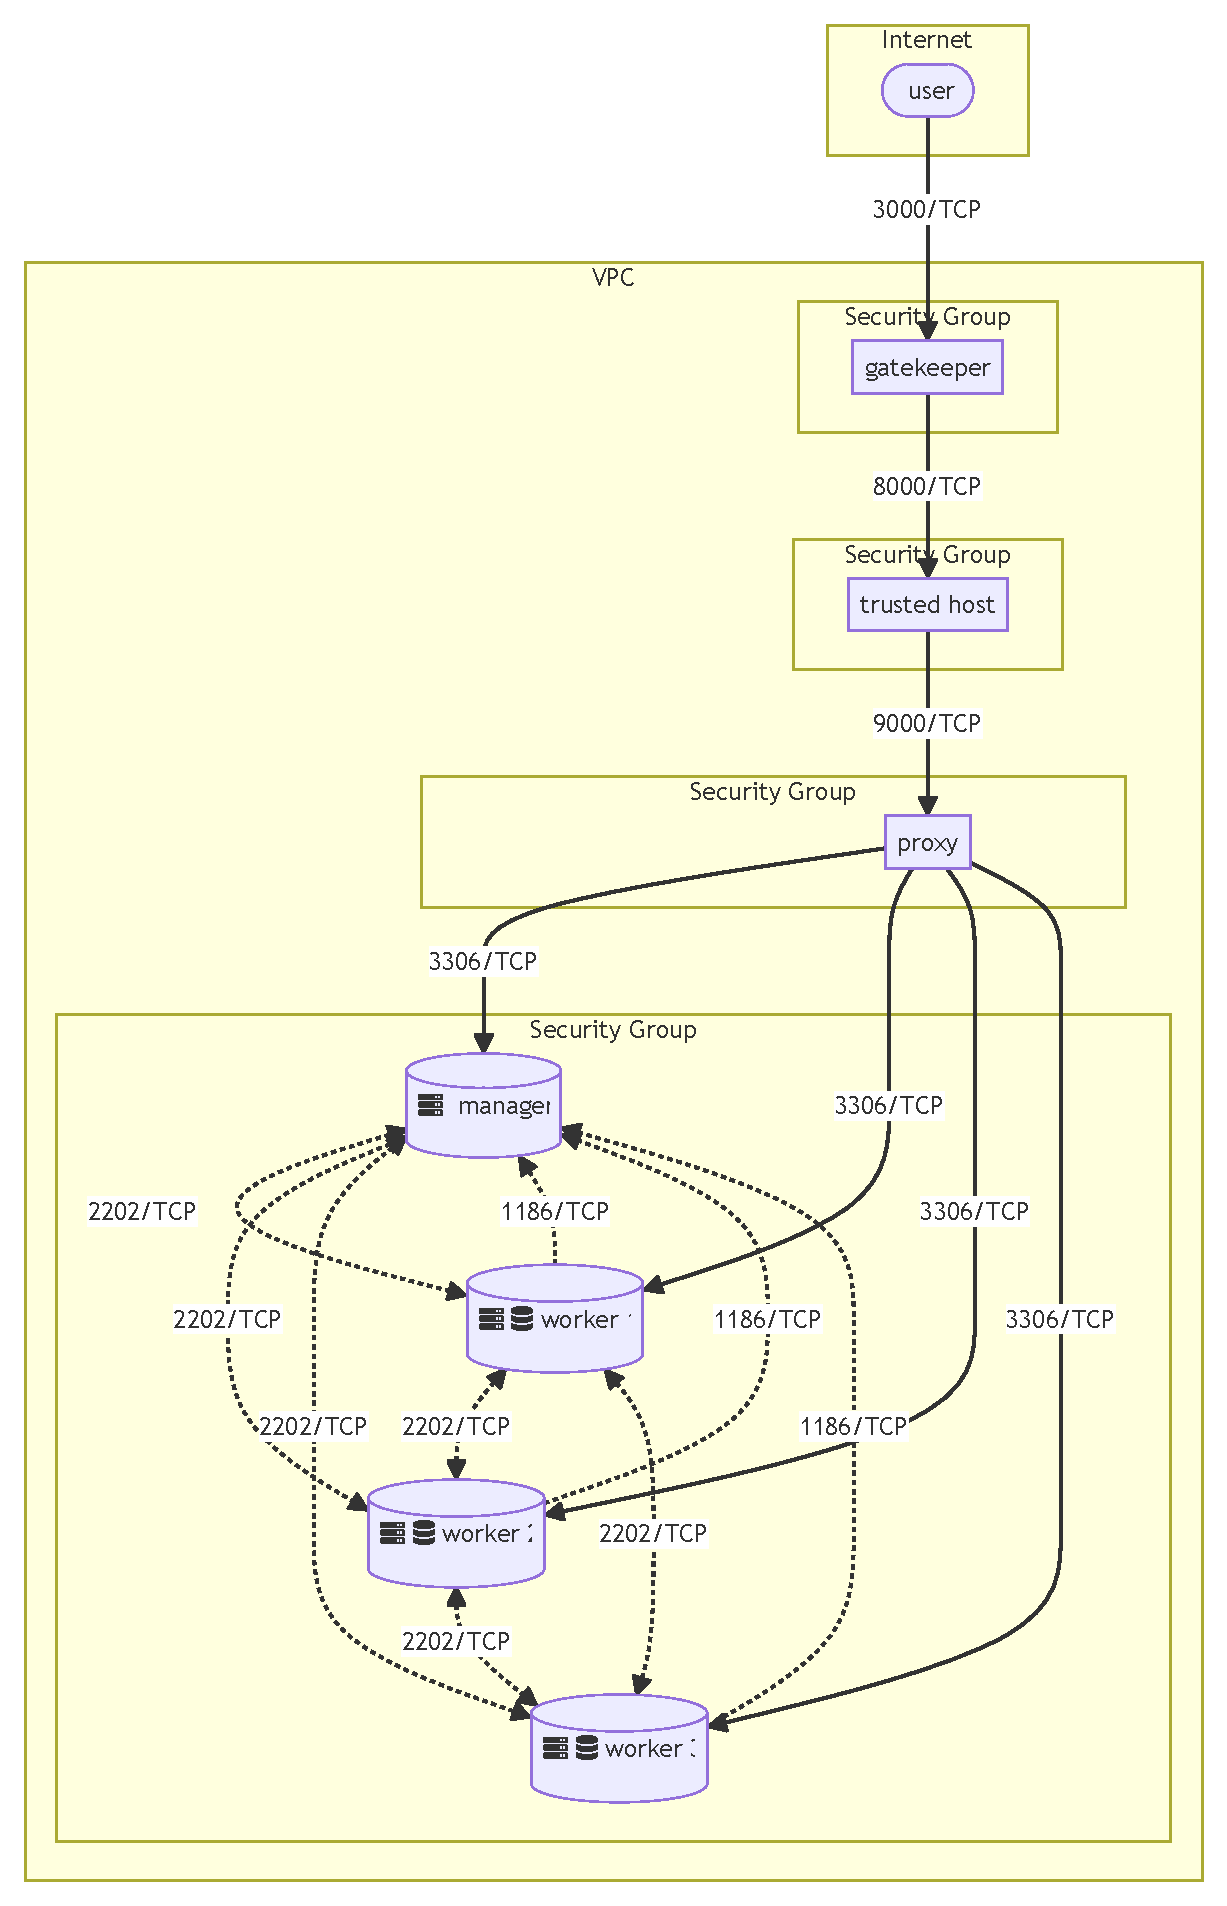
\includegraphics[width=0.75\linewidth]{figures/patterns.mmd.pdf}
    \caption{Cloud patterns}
    \label{fig:patterns}
\end{figure}

To offer better read scalability and security, we implement two Cloud patterns: Proxy and Gatekeeper. Proxy will act as a "smart" load balancer between the client and the database cluster nodes while Gatekeeper will help minimize the attack surface by filtering the incoming traffic.

Figure~\ref{fig:patterns} shows the complete architecture of the project with the cluster behind a Proxy and a Gatekeeper.

\subsubsection{Proxy}

\textbf{File: \texttt{src/patterns/apps/proxy.ts}}

The proxy is a Deno (\url{https://deno.com}) TypeScript application that offers a simple REST API to query the database. 3 (POST) routes are available:

\begin{itemize}
    \item \texttt{/direct}: Direct hit, all requests are forwarded to the master
    \item \texttt{/random}: Random hit, one slave is randomly selected
    \item \texttt{/customized}: Measure the latency of each node and select the fastest one
\end{itemize}

If the query is a write statement (e.g. \texttt{INSERT}, \texttt{UPDATE}, \texttt{DELETE}), the request is always replicated to all nodes and the response from the master is returned to the client.

\subsubsection{Gatekeeper}

\textbf{Files: \texttt{src/patterns/apps/\{gatekeeper,trusted\}.ts}}

Gatekeeper is composed of two instances, one public-facing (referred to as "gatekeeper") and one private (referred to as "trusted host").

They both also run Deno TypeScript applications. The gatekeeper forwards all incoming requests to the trusted host that will sanitize the query and forward it to the proxy. The response is then returned to the client.

\subsubsection{Security Considerations}

We use multiple security groups to restrict the access to the different instances:

\begin{itemize}
    \item The cluster security group allows all internal traffic from the 4 instances and the traffic from the proxy on port 3306 (mysqld).
    \item The proxy security group only allows incoming traffic from the trusted host on port 9000 (Deno Proxy application).
    \item The trusted host security group only allows incoming traffic from the gatekeeper on port 8000 (Deno Trusted Host application).
    \item The gatekeeper security group allows all incoming traffic from the Internet on port 3000 (Deno Gatekeeper application).
\end{itemize}

We also use the internal IP addresses of the instances to communicate between them inside the VPC.

The trusted host is responsible for sanitizing the incoming queries to prevent SQL injections. Because we allow any query to be executed on the database, we cannot use prepared statements to prevent this kind of attack. Instead, we rely on a simple regular expression to filter out the dangerous characters. It is far from a perfect solution but it is enough for the scope of this project.

\clearpage
\section{Results and Outcomes}

\subsection{MySQL deployments}

\subsubsection{Standalone server}

Once the deployment is complete, we can simply connect to the database using the \texttt{mysql} command-line client. Figure~\ref{fig:standalone_query} shows a simple query on the loaded \texttt{sakila} database.

\begin{figure}[h]
    \centering
    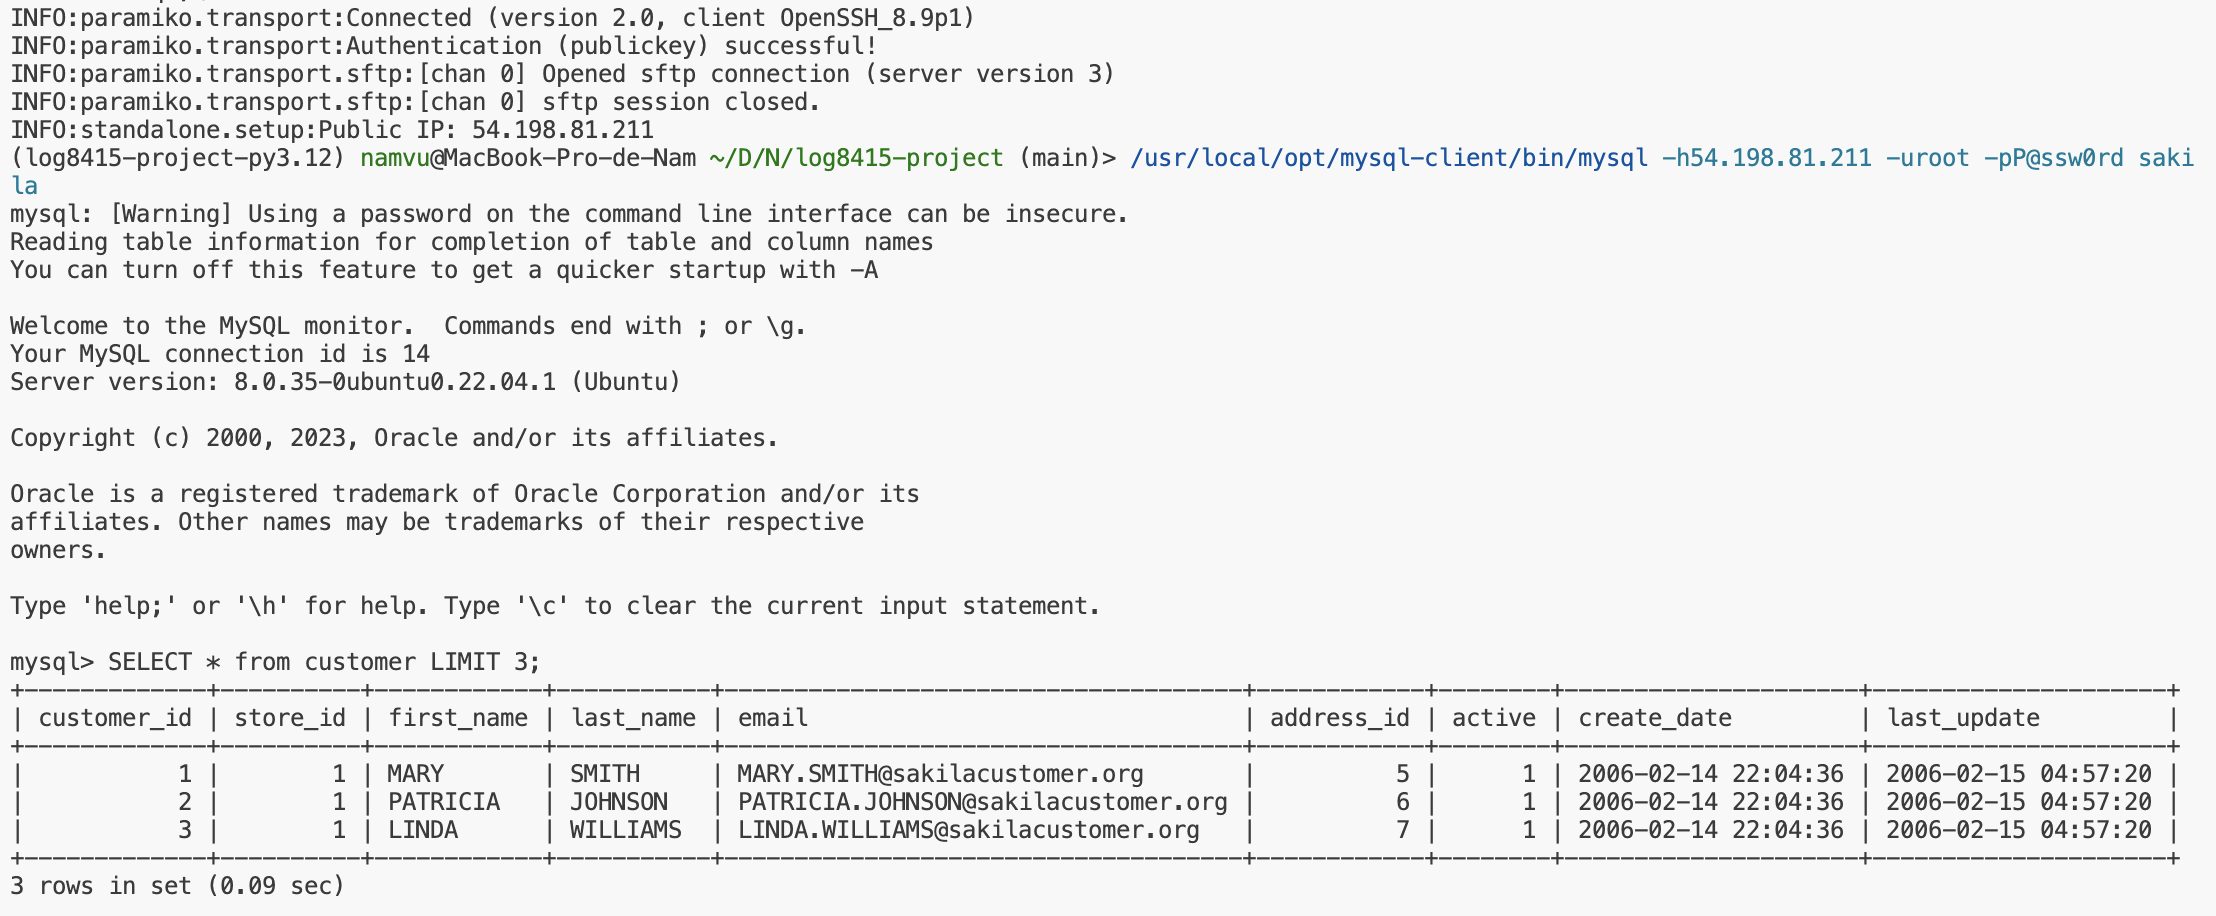
\includegraphics[width=\linewidth]{figures/Screenshot 2023-12-25 at 16.16.05.png}
    \caption{Standalone query}
    \label{fig:standalone_query}
\end{figure}

\subsubsection{Cluster}

Figure~\ref{fig:ndb_mgm} shows a deployed cluster infos: here we have 172.31.95.195 as the manager node (coordinator, \texttt{ndb\_mgmd}) and 172.31.28.31, 172.31.40.222 and 172.31.6.155 as worker nodes (responsible for storing data, \texttt{ndbd}). Every node exposes the MySQL API (\texttt{mysqld}) that can be accessed on their respective port 3306.

\begin{figure}[h]
    \centering
    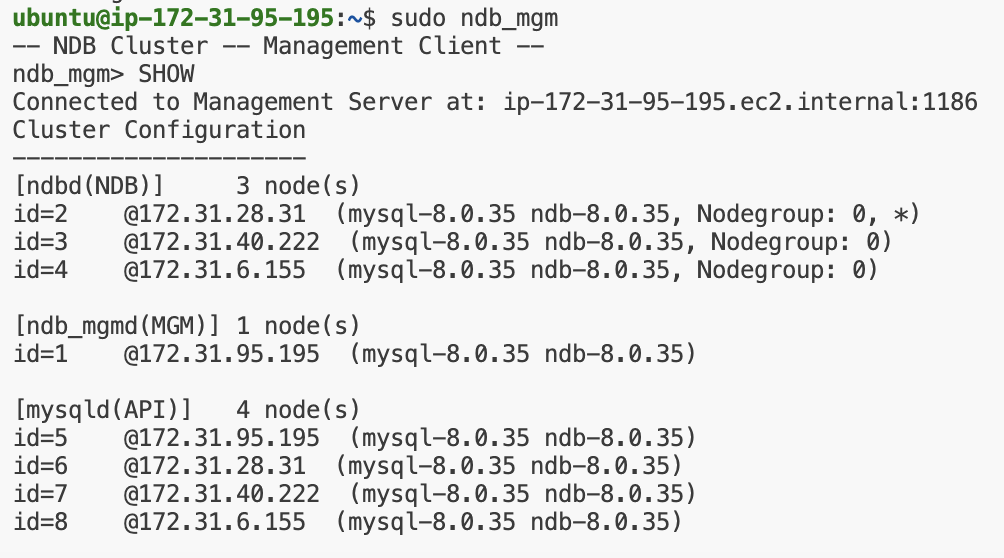
\includegraphics[width=0.5\linewidth]{figures/Screenshot 2023-12-24 at 21.30.58.png}
    \caption{Cluster informations}
    \label{fig:ndb_mgm}
\end{figure}

\subsection{Benchmarking}

We ran \texttt{tools/benchmark.sh} on both standalone and cluster deployments (we benchmarked the master of the later). The results are shown respectively in Figures~\ref{fig:standalone_benchmark} and \ref{fig:cluster_benchmark}.

The cluster deployment appear to be slightly slower than the standalone server (2941.76 vs 3072.47 queries per second). This can be due to the overhead of the cluster management and the network latency between the manager and worker nodes.

\begin{figure}[h]
    \centering
    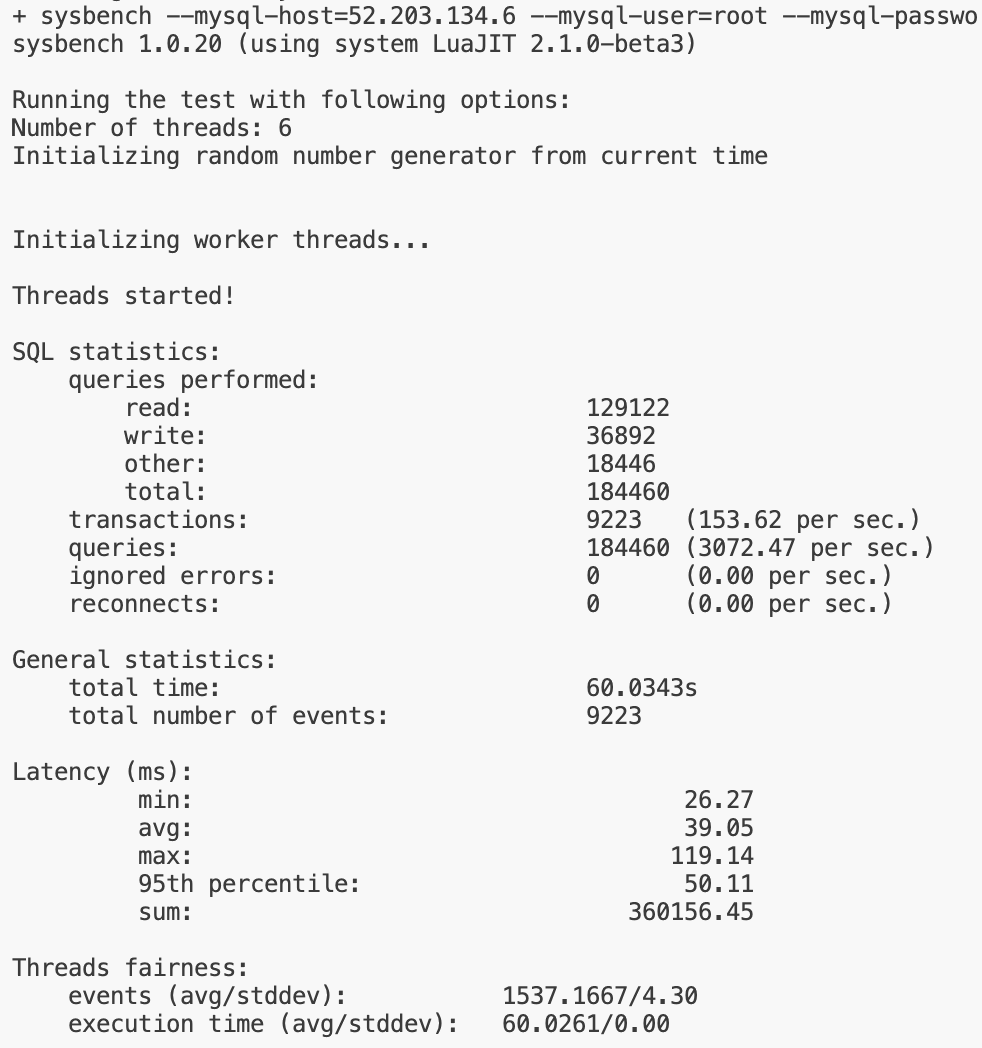
\includegraphics[width=0.75\linewidth]{figures/Screenshot 2023-12-25 at 16.42.56.png}
    \caption{Standalone benchmark}
    \label{fig:standalone_benchmark}
\end{figure}

\begin{figure}[h]
    \centering
    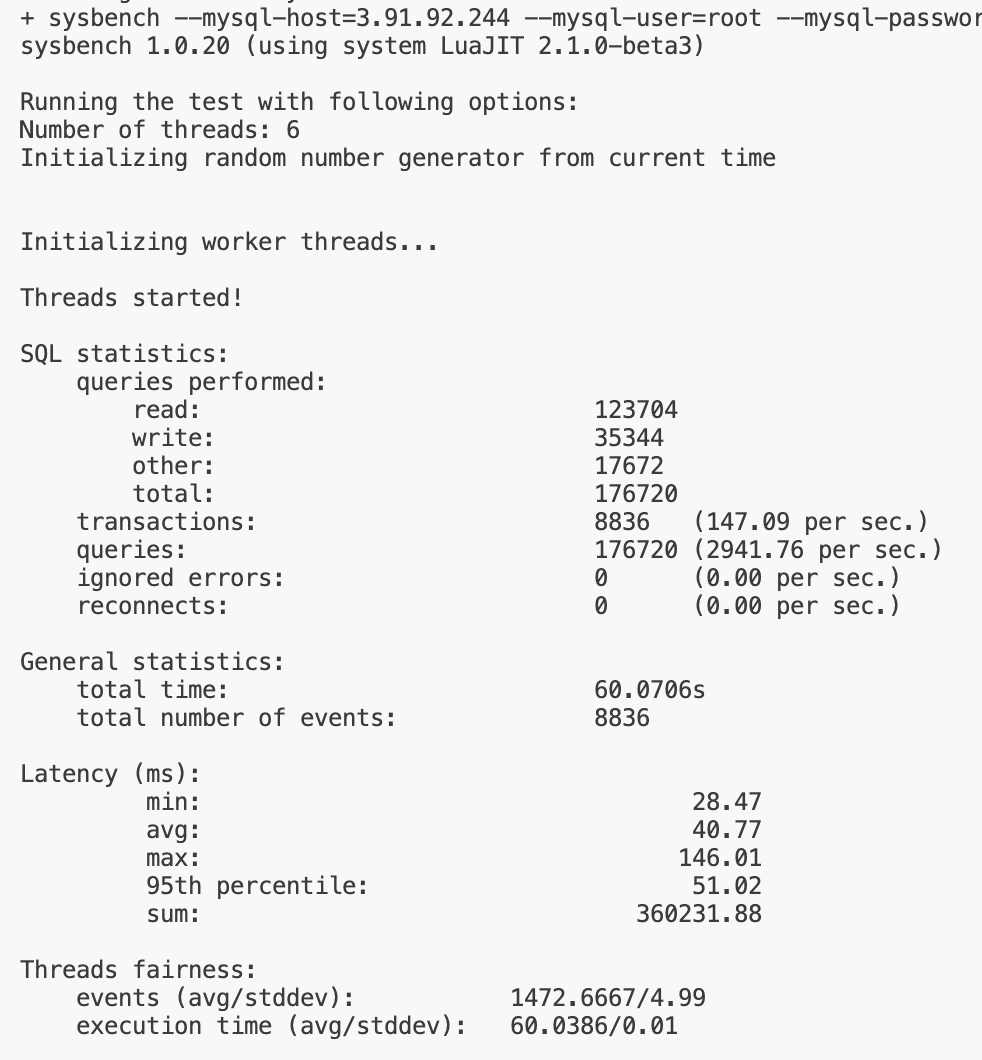
\includegraphics[width=0.75\linewidth]{figures/Screenshot 2023-12-25 at 16.53.44.png}
    \caption{Cluster benchmark}
    \label{fig:cluster_benchmark}
\end{figure}

\clearpage
\subsection{Cloud patterns}

The patterns module deploys a cluster (Figure~\ref{fig:patterns_cluster}) behind a proxy, a trusted host and a gatekeeper.

The gatekeeper is accessible from the Internet on port 3000. It receives POST requests from the client on \texttt{/direct}, \texttt{/random} and \texttt{/customized} routes with the query in the body (\texttt{query} field). After forwarding to the trusted host and proxy, the cluster response is returned back to the client.

\begin{figure}[h]
    \centering
    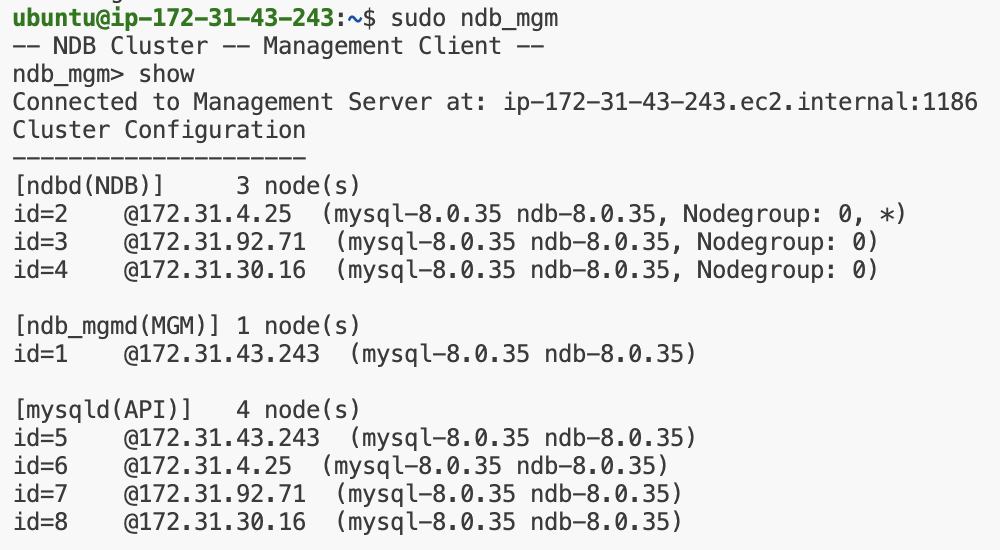
\includegraphics[width=0.75\linewidth]{figures/Screenshot 2023-12-25 at 23.18.08.png}
    \caption{Patterns cluster}
    \label{fig:patterns_cluster}
\end{figure}

Sample requests are shown in Figures~\ref{fig:patterns_random}, \ref{fig:patterns_direct} and \ref{fig:patterns_customized}. The first request is a read only query (\texttt{SELECT}) on \texttt{/random} that will be forwarded to a random worker node. The second request is a write query (\texttt{INSERT}) on \texttt{/direct} that will be replicated to all nodes (the response is the one from the master). The third request is a read only query (\texttt{SELECT}) on \texttt{/customized} that will be forwarded to the fastest node (according to ping time). This last query confirms that our previous write was successfully replicated to all nodes.

\begin{figure}[h]
    \centering
    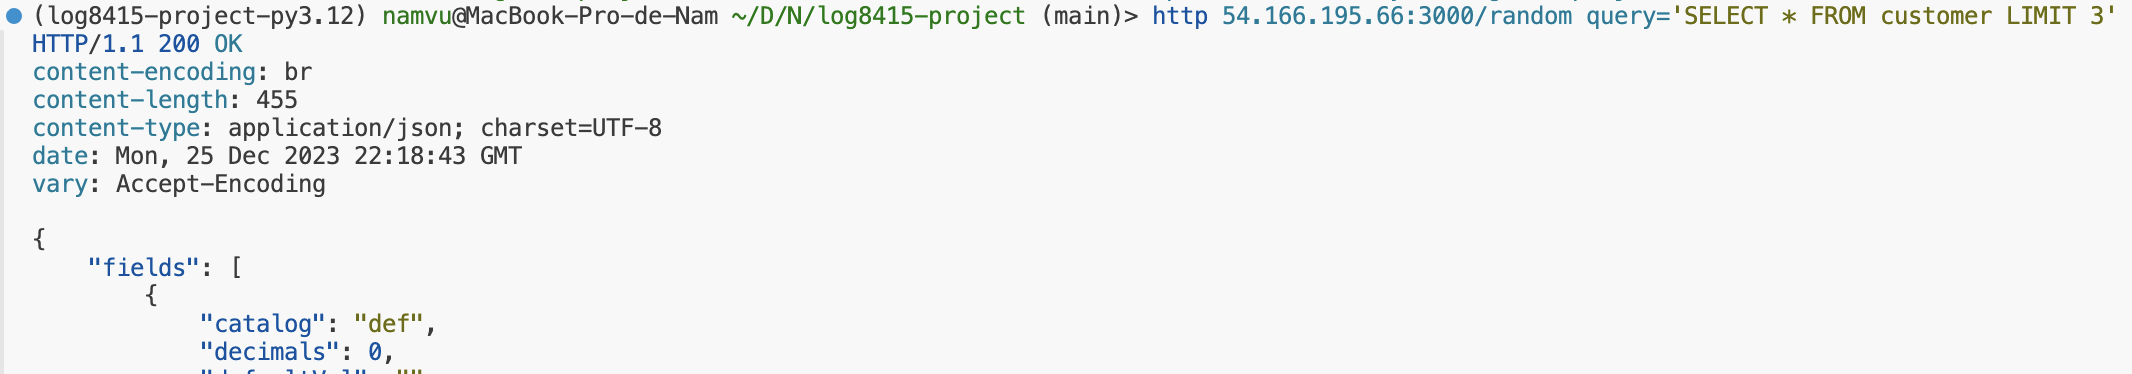
\includegraphics[width=\linewidth]{figures/Screenshot 2023-12-25 at 23.20.43.png}
    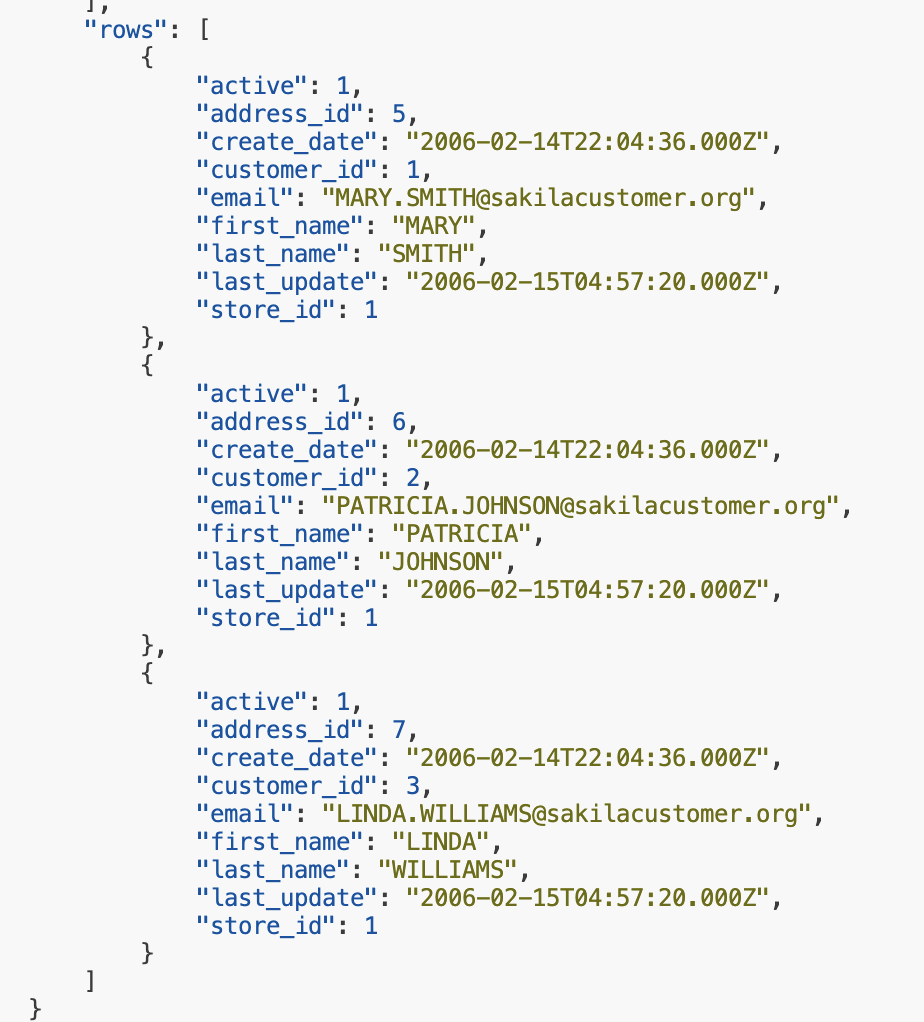
\includegraphics[width=0.75\linewidth]{figures/Screenshot 2023-12-25 at 23.20.52.png}
    \caption{Gatekeeper request (SELECT, \texttt{/random})}
    \label{fig:patterns_random}
\end{figure}

\begin{figure}[h]
    \centering
    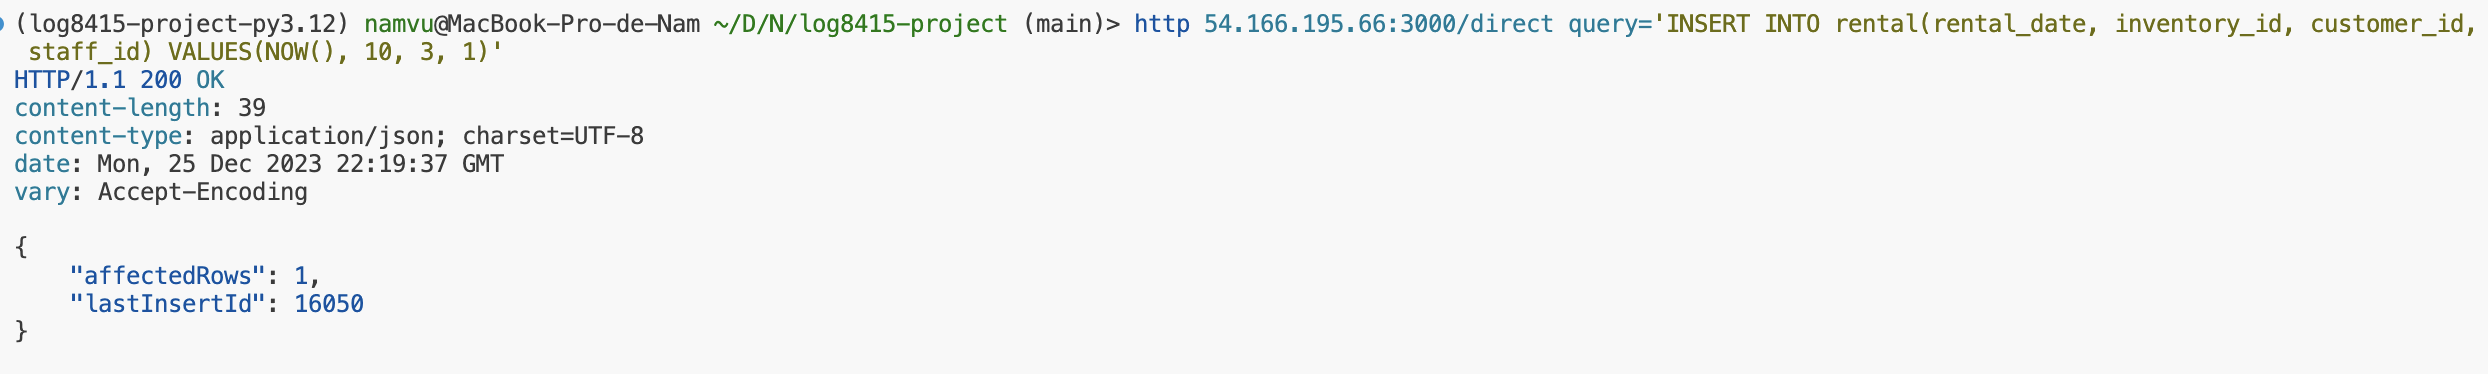
\includegraphics[width=\linewidth]{figures/Screenshot 2023-12-25 at 23.21.17.png}
    \caption{Gatekeeper request (INSERT, \texttt{/direct})}
    \label{fig:patterns_direct}
\end{figure}
\begin{figure}[h]
    \centering
    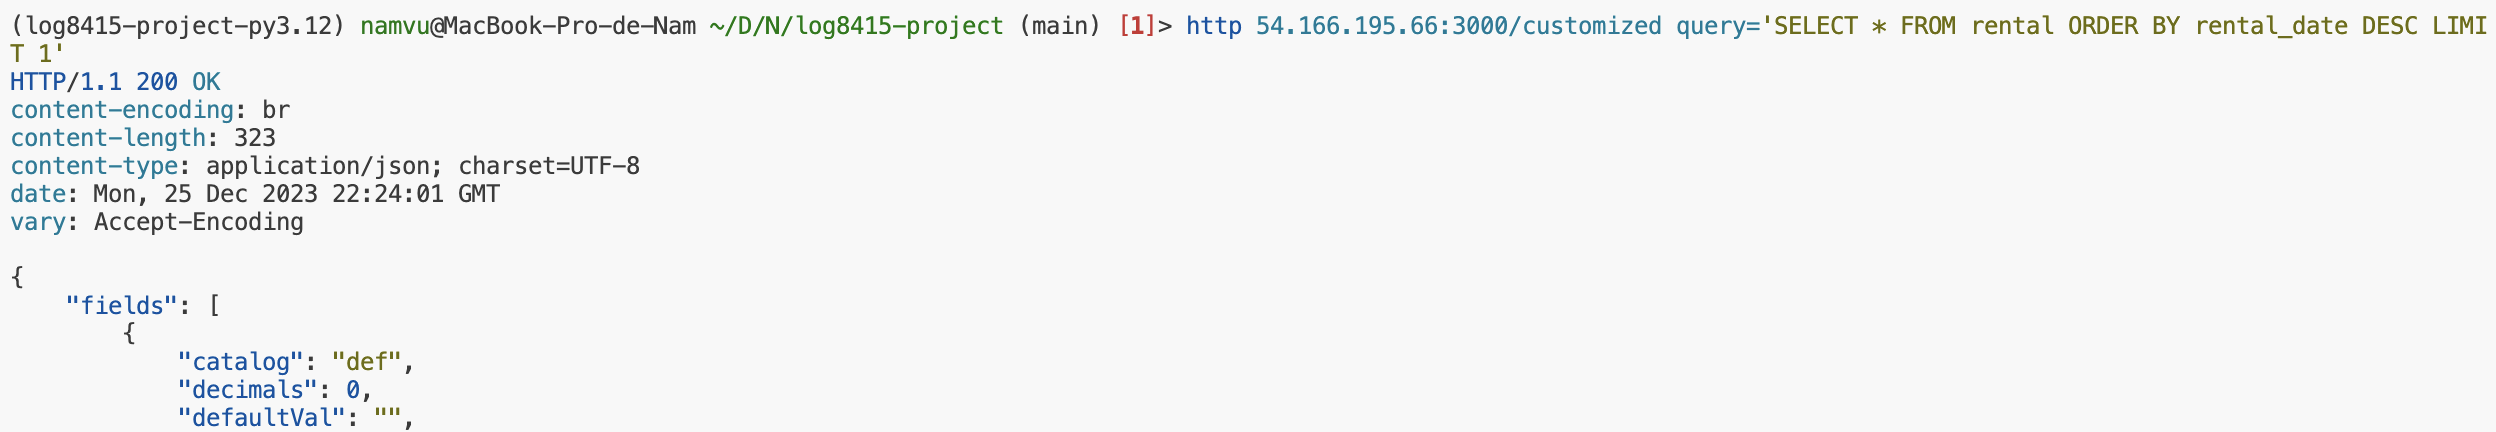
\includegraphics[width=\linewidth]{figures/Screenshot 2023-12-25 at 23.24.17.png}
    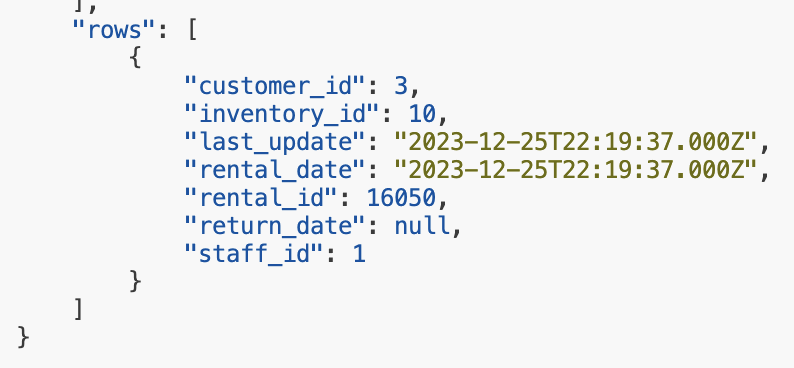
\includegraphics[width=0.75\linewidth]{figures/Screenshot 2023-12-25 at 23.24.23.png}
    \caption{Gatekeeper request (SELECT, \texttt{/customized})}
    \label{fig:patterns_customized}
\end{figure}

Figure~\ref{fig:patterns_logs} shows the logs of the different components. We can see that the gatekeeper (left) receives the first request on \texttt{/random} and forwards it to the trusted host. The trusted host (middle) sanitizes the query and then forwards it to the proxy (right) that chooses a random worker to execute this read only query. The second query on \texttt{/direct} is a write query that is replicated to all nodes. Finally, the third query on \texttt{/customized} requires the proxy to ping all nodes and select the fastest one to execute the query.

\begin{figure}[h]
    \centering
    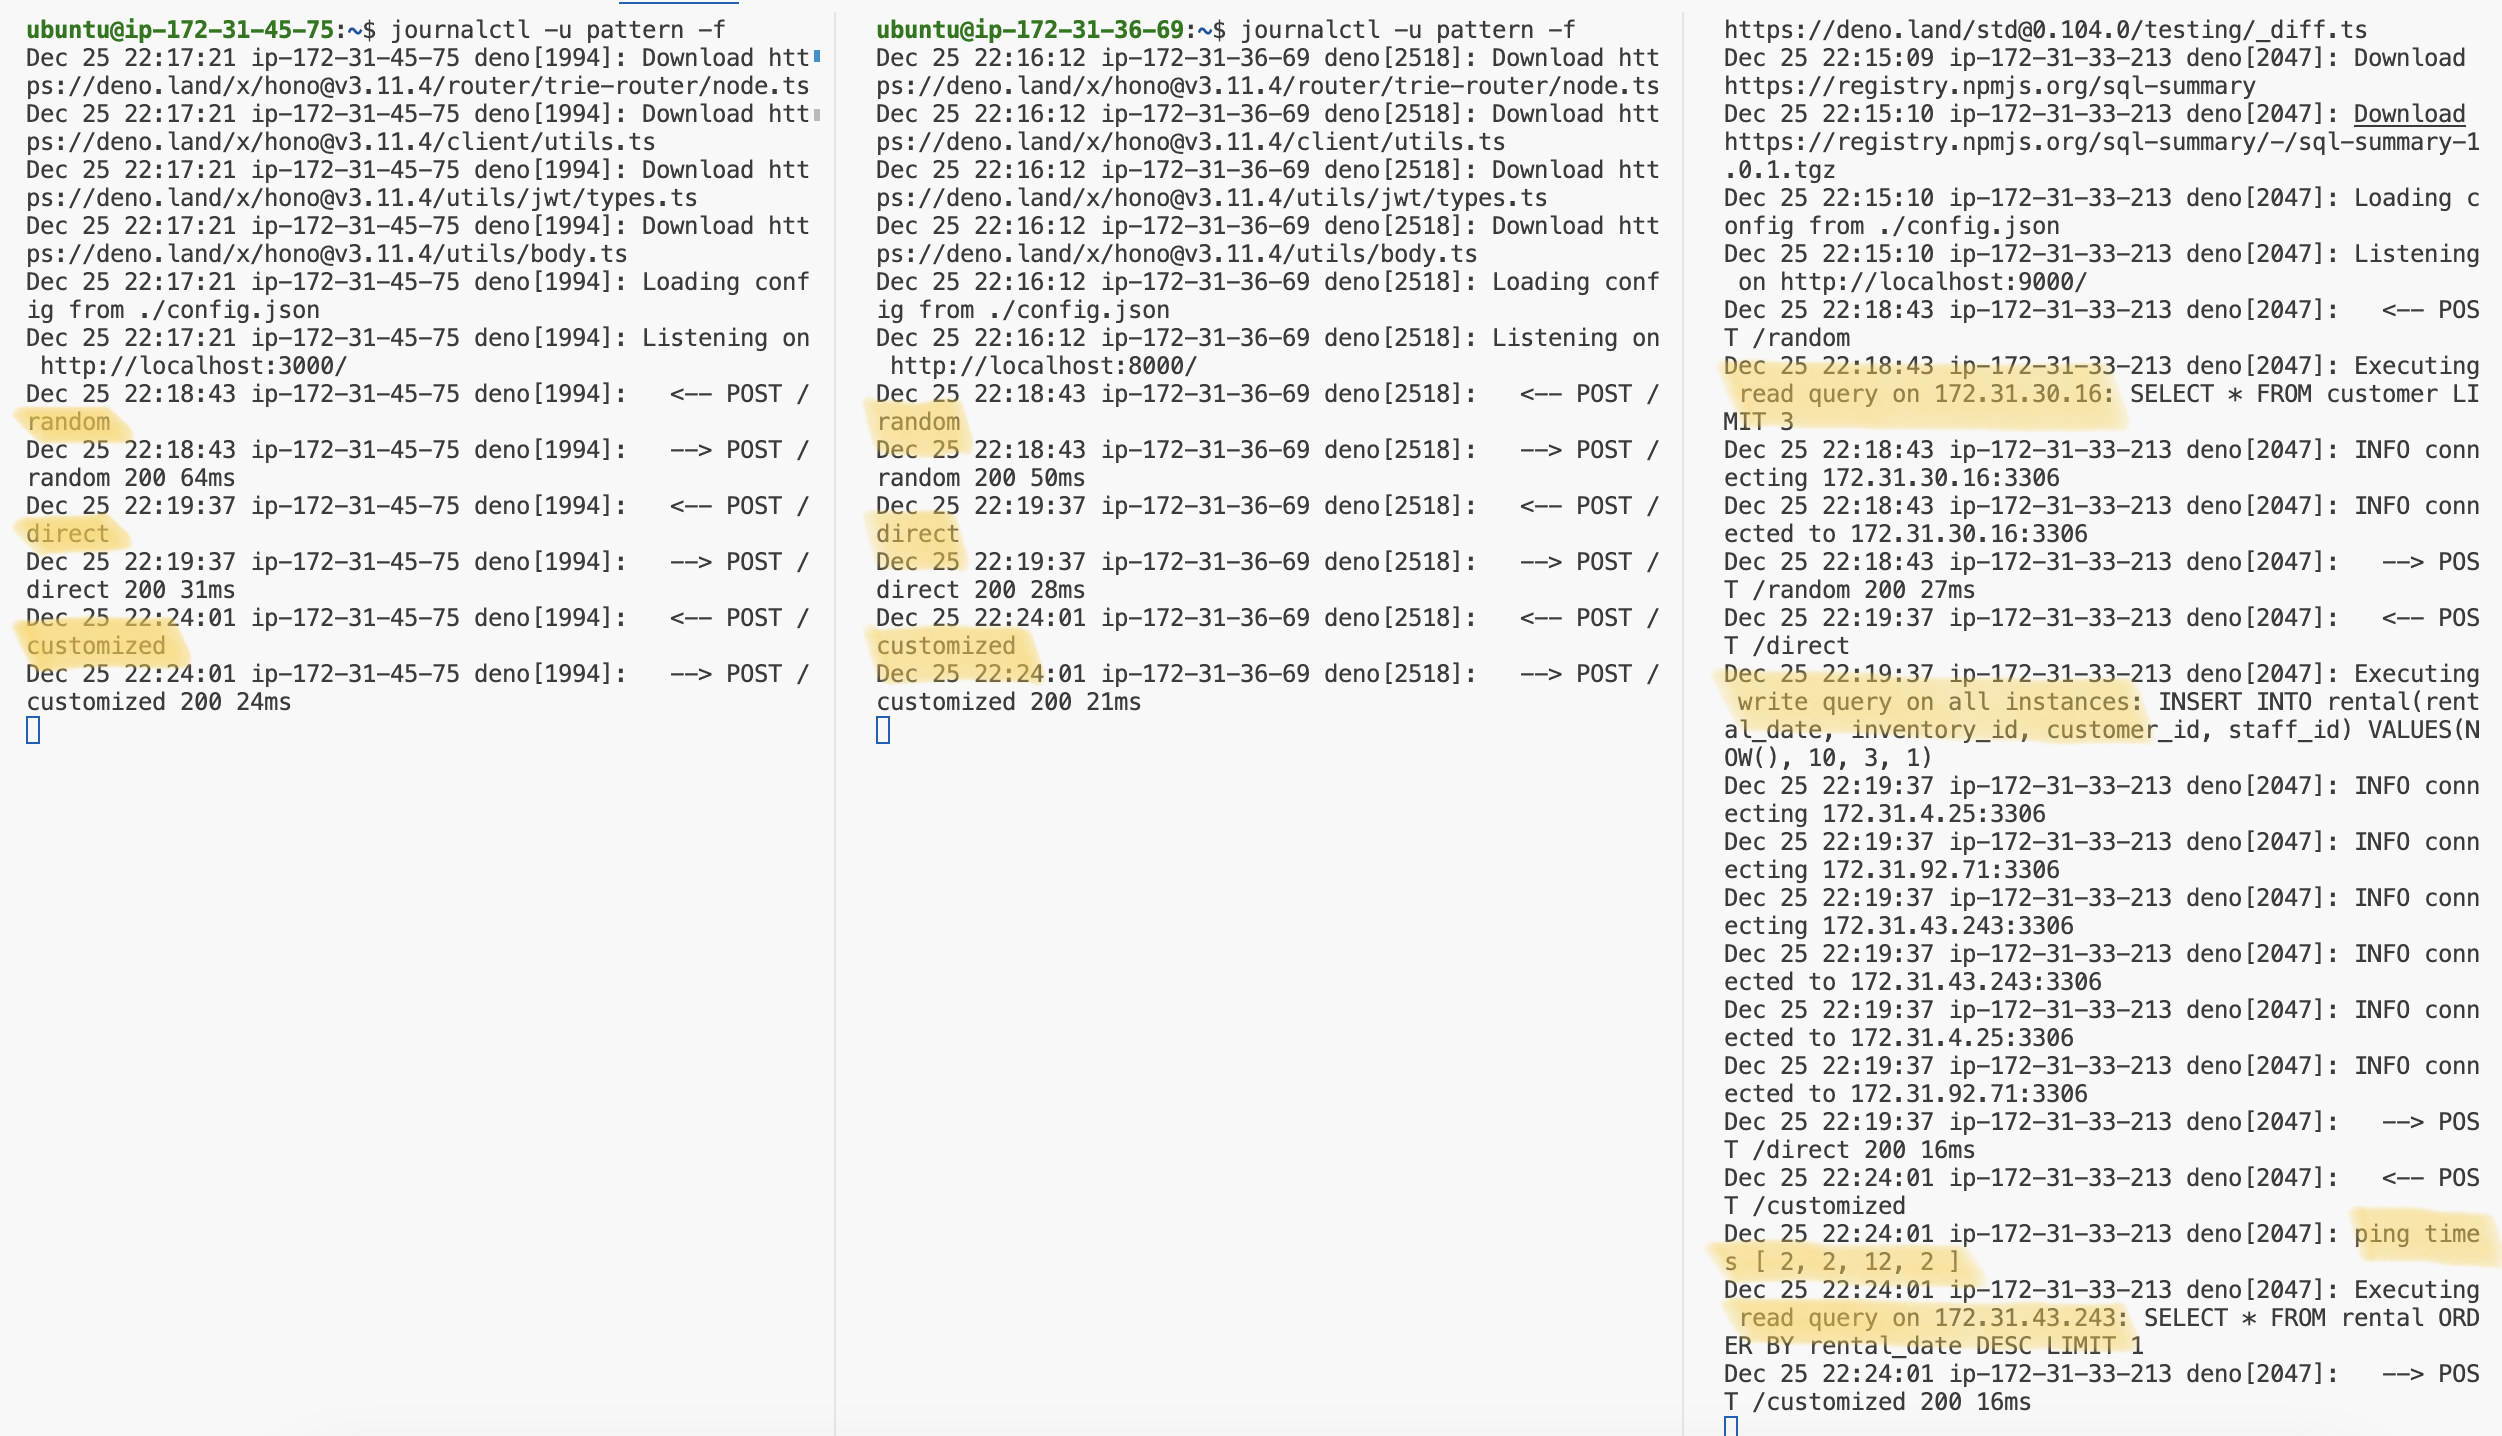
\includegraphics[width=\linewidth]{figures/Screenshot 2023-12-25 at 23.24.34.png}
    \caption{Patterns apps logs (gatekeeper, trusted host, proxy)}
    \label{fig:patterns_logs}
\end{figure}

\clearpage
\section{Lessons Learned}

\begin{itemize}
    \item You better just go through the official ugly documentation of MySQL instead of relying on pretty but outdated third-party tutorials to set up things properly.
    \item Security groups are an easy and efficient way to restrict the access to the instances.
    \item Templates are very useful to dynamically generate configuration files for multiple instances.
\end{itemize}

\section{Recommendations}

\begin{itemize}
    \item The \textit{sakila} example database is not meant to be used in a (NDB) cluster: it relies on the \texttt{InnoDB} engine that is not the one provided by the MySQL NDB Cluster (\texttt{NDBEngine}). That makes this database loaded into the instance locally and not replicated across the three workers. As a consequence for this assignement, we had to manually load the database on the manager and each worker node and rely on the Proxy to replicate the write queries to all nodes (\texttt{NDBEngine} should have done that automatically).
    \item The proxy can be improved to detect \texttt{mysqld} failures and automatically remove the instance from the pool of available nodes.
    \item The Gatekeeper, the Trusted Host and the Proxy can be scaled horizontally to improve the availability of the system (in the current configuration if one of the three instances fails, the whole system is down).
\end{itemize}

\section{Conclusion}

In this project, we were able to efficiently setup a MySQL cluster on Amazon EC2 and implement two Cloud patterns: Proxy and Gatekeeper. Security concerns were also addressed by restricting the access to the instances and sanitizing the incoming queries. Finally, we benchmarked the performance of the two deployments and found that the cluster was slightly slower than the standalone server.

All the code was developed in Python and TypeScript while keeping in mind performance (\texttt{asyncio} concurrency) and maintenability (modularity, reusability). That allowed us from the start to easily extend the previous projects codebase and implement the new features required for this assignment.

\addsec{Attachments}

\subsection*{Git Repository}

\url{https://github.com/NextFire-PolyMTL/log8415-project}

List of authors:

\begin{itemize}
    \item Nam Vu: \texttt{NextFire <git@yuru.moe>}
\end{itemize}

\subsection*{Demo Video}

\url{https://drive.google.com/file/d/1eNEslekpXstN5InSCTaYVMzah81akDhY/view}

0:00-12:30 Code walkthrough, 12:30-end Execution demo

Changes since the recording:

\begin{itemize}
    \item (proxy) Manager node is now included in the considered instances for the \texttt{/customized} route (as required by the assignment)
    \item (proxy) The full response object from the cluster is now returned (instead of only the \texttt{rows} field). This is reflected in the Figures~\ref{fig:patterns_random}, \ref{fig:patterns_direct} and \ref{fig:patterns_customized}.
\end{itemize}

\addsec{Signatures}

Nam V.

% \printbibliography

\end{document}
